\chapter{Вывод в Марковских Случайных Полях} \label{chap:mrf}
\section{Марковскиe Случайныe Поля} \label{sec:mrf}

Рассмотрим гиперграф $\mathcal{G} = (\mathcal{V}, \mathcal{E})$ с конечным множеством вершин~$\mathcal{V}$ и гиперебер~$\mathcal{E}$.
Пусть все вершины пронумерованы от~$1$ до~$n$, а все гиперребра от~$1$ до~$m$.

Сопоставим каждой вершине~$k = 1,\ldots,d$ переменную~$x_k$ принимающую значения из множества $\mathcal{X}_k = \{1,\dots,n_k\}$.
Обозначим множество вершин, входящих в гиперребро~$\ell = 1, \ldots, m$, через ~$\vec{x}^\ell$.
Каждому гиперребру~$\ell = 1, \ldots, m$ сопоставим вещественнозначную функцию~$\Theta_\ell$, определенную на совместной области определения переменных из~$\vec{x}^\ell$: $\Theta_\ell: \prod_{k=1}^d \mathcal{X}_k \to \mathcal{R}$. Функцию~$\Theta_\ell$ будем называть \emph{потенциалом}.

\emph{Функцией энергии} марковского случайного поля (Markov random field, MRF) заданного на гиперграфе~$\mathcal{G}$, назовем сумму всех потенциалов:
$
E(\vec{x}) = \sum_{\ell = 1}^{m} \Theta_\ell(\vec{x}^{\ell}).
$

Экспонента от минус энергии задает \emph{ненормированное распределение Гиббса}:
$
\widehat{P}(\vec{x}) = \exp(-E(\vec{x})).
$
Для обозначения нормировочной константы будет использоваться символ~$Z$, $Z = \sum_{\vec{x}} \widehat{P}(\vec{x})$. Функции $\Psi_\ell(\vec{x}^\ell) = \exp(-\Theta_\ell(\vec{x}^{\ell}))$ будем называть \emph{факторами} марковского случайного поля.

Как энергия, так и ненормированная вероятность являются $d$-мерными тензорами. Потенциалы и факторы можно интерпретировать как $d$-мерные тензоры, если добавить в них переменные, от которых они зависят несущественно: $\tensGreek{\Theta}_\ell (\vec{x}^\ell) = \tensGreek{\Theta}_\ell (\vec{x})$. Тензоры энергии и вероятности можно определить следующим образом:
$
\tens{E} = \sum_{\ell = 1}^m \tensGreek{\Theta}_\ell
$
и
$
\widehat{\tens{P}} =   \bigodot_{\ell = 1}^m \tensGreek{\Psi}_\ell.
$

Таким образом, марковское случайное поле с помощью потенциалов с настраиваемыми параметрами задает вероятностное распределение над $d$-мерным вектором $\vec{x}$. Аппарат марковских случайных полей используют для решения задач машинного обучения со структурированными данными. Например, при необходимости решения задачи семантической сегментации изображений (см. Рис.~\ref{fig:segmentation} \alert{TODO}) ставится задача по определению класса каждого пикселя (классификации). Однако при решении данной задачи независимо для каждого пикселя, изображение результат получается низкого качества, так как информация о разметке одного пикселя несет информацию о разметке соседних пикселей и предположение об условной независимости не выполняется на практике (см. Рис.~\ref{fig:segmentation}б \alert{todo}). При решении задачи семантической сегментация с помощью МРФ данные зависимости не игнорируются, и моделируется вероятностное распределение $P(\vec{x} \mid \vec{h})$, где $d$-мерный вектор $\vec{x}$ задает один из $n$ классов в каждом из $d$ пикселей, а $\vec{h}$ кодирует информацию об обрабатываемом изображении, например яркость каждого из $d$ пикселей. Для задачи семантической классификации часто используют (гипер)-граф типа решетка (см. Рис.~\ref{fig:mrf-graph} \alert{todo}). Потенциалы при этом могут задаваться следующим образом: \emph{унарные потенциалы} (то-есть потенциалы зависящие только от одной переменной для каждого пикселя) $\tensGreek{\Theta}_k(x_k)$ задают логарифм уверенности базового классификатора в том, что $k$-ый пиксель принадлежит классу $x_k$, а бинарные потенциалы заданные на ребрах графа $\tensGreek{\Theta}_{k_i, k_j}(x_{k_i}, x_{k_j})$ задают априорные представления о корреляции меток в соседних пикселях (например потенциал Поттса $\tensGreek{\Theta}_{k_i, k_j}(x_{k_i}, x_{k_j}) = [x_{k_i} \neq x_{k_j}]$ штрафует модель за слишком большое количество границ между классами)~\cite{some mrf segmentaion}. Задав модель марковского случайного поля можно, например, использовать метод максимума правдоподобия для её обучения, то-есть максимизировать правдоподобие обучающей выборки $(\vec{h}^{(f)}, \vec{x}^{(f)})_{f=1}^N$ по параметрам $\vec{w}$
$$
\max_{\vec{w}} \prod_{f=1}^N \frac{1}{Z(\vec{w}, \vec{h}^{(f)})}\exp(-\sum_{\ell=1}^m\tensGreek{\Theta}(\vec{x}^{(f)}, \vec{h}^{(f)}, w))
$$
где нормировочная константа $Z(w)$ определяется как сумма по экспоненциально большому числу возможных сегментаций
$$
Z(w, \vec{h}) = \sum_{\vec{x}}\exp(-\sum_{\ell=1}^m\tensGreek{\Theta}(\vec{x}, \vec{h}, \vec{w}))
$$

Таким образом, одна из главных задач в теории и практике применения марковских случайных полей это приближенный подсчет нормировочной константы $Z$. Обратим внимание на то, что точной подсчет нормировочной константы МРФ в общем случае является NP-сложной задачей~\cite{todo}.

После обучения, применять модель марковского случайного поля можно находя разметку наибольшей вероятности для данного изображения $\vec{h}$
$$\argmax_{\vec{x}} \frac{1}{Z(\vec{w}, \vec{h})}\exp(-\sum_{\ell=1}^m \tensGreek{\Theta}(\vec{x}, \vec{h}, \vec{w})) = \argmin \sum_{\ell=1}^m\tensGreek{\Theta}(\vec{x}, \vec{h}, \vec{w})$$	
Другой способ применение обученного МРФ к новым изображениям это вычисление значения \emph{маргинальных распределений}, тоесть распределений на сегментацию отдельных пикселей получамых из условной вероятности на сегментацию всех пикселей путем суммирования по всем пикселям кроме данного
$$
p(x_k \mid \vec{h}, \vec{w}) = \sum_{x_1=1}^n \ldots \sum_{x_{k-1}=1}^n\sum_{x_{k+1}=1}^n \ldots \sum_{x_{d}=1}^n p(\vec{x} \mid \vec{h}, \vec{w})
$$

Таким образом, задачи дискретной минимазации энергии заданной в виде суммы потенциалов, а задачи подсчета маргинальных распределений, так же являются важнейшими для использования МРФ на практике.

\section{Основные подходы к задаче вывода} \label{sec:mrf-approaches}

Существует две основных постановки задачи вывода в графической модели: минимизация энергии и вероятностный вывод.
На текущий момент, задача минимизации энергии хорошо изучена. В последних экспериментальных исследованиях Каппес и др. показывают~\cite{Kappes13comparison}, что для многих актуальных задач текущие методы дают достаточно хорошие результаты. Особенно много внимания уделено парно-сепарабельным марковским случайным полям (см. детальный обзор Каппеса и др.~\cite{Kappes13comparison}).
Под вероятностным выводом понимается множество различных задач. В данной диссертации уделено внимание двум из них: вычислению нормировочной константы по ненормированному распределению марковского случайного поля и вычислению маргинальных распределений.
Вторая проблема является более сложной, так как для её решения зачастую требуется вычисление нормировочной константы.

Можно выделить следующие группы методов подсчета нормировочной константы: методы, основанные на генерации выборки (например~Annealed Importance Sampling~\cite{neal01ais,grosse13}), методы передачи сообщений (классический Loopy Belief Propagation~\cite{kschischang01bp} и его многочисленные модификации), методы, основанные на минимизации KL\hyp{}дивергенции (Mean Field~\cite{wainwright08gm} и Expectation Propagation~\cite{minka04treeep}), методы декомпозиции графов (Tree\hyp{}Reweighted Message-passing~\cite{wainwright05trw}) и методы, основанные на минимизации энергии (randomized MAP\hyp{}predictors~\cite{hazan13} и недавно предложенный метод WISH~\cite{ermon13wish}).
Для решения задачи вычисления маргинальных распределений подходят более простые методы, такие как Gibbs sampling~\cite{wainwright08gm}.

\section{Тензорный алгоритм вывода} \label{sec:tt-mrf}
\subsection{Тензоры марковского случайного поля} \label{sec:mrf-as-tensor}

\begin{figure}
\vskip 0.2in
\begin{center}
\resizebox{0.8\columnwidth}{!}{
\begin{tikzpicture}[>=latex',line join=bevel,]
	\tikzstyle{every node}=[font=\fontsize{25}{1}]
  \pgfsetlinewidth{1bp}
%%
\pgfsetcolor{black}
  % Edge: a_0 -- G_1
  \draw [] (56.23bp,18bp) .. controls (62.06bp,18bp) and (67.889bp,18bp)  .. (73.719bp,18bp);
  % Edge: dots -- G_n
  \draw [] (346bp,18bp) .. controls (351.98bp,18bp) and (357.95bp,18bp)  .. (363.93bp,18bp);
  % Edge: G_2 -- dots
  \draw [] (274bp,18bp) .. controls (279.98bp,18bp) and (285.95bp,18bp)  .. (291.93bp,18bp);
  % Edge: G_1 -- a_1
  \draw [] (128.09bp,18bp) .. controls (133.95bp,18bp) and (139.81bp,18bp)  .. (145.66bp,18bp);
  % Edge: x_n -- G_n
  \draw [] (391bp,71.831bp) .. controls (391bp,61bp) and (391bp,47.288bp)  .. (391bp,36.413bp);
  % Edge: G_n -- a_n
  \draw [] (418.09bp,18bp) .. controls (423.95bp,18bp) and (429.81bp,18bp)  .. (435.66bp,18bp);
  % Edge: x_1 -- G_1
  \draw [] (101bp,71.831bp) .. controls (101bp,61bp) and (101bp,47.288bp)  .. (101bp,36.413bp);
  % Edge: x_2 -- G_2
  \draw [] (247bp,71.831bp) .. controls (247bp,61bp) and (247bp,47.288bp)  .. (247bp,36.413bp);
  % Edge: a_1 -- G_2
  \draw [] (202.23bp,18bp) .. controls (208.06bp,18bp) and (213.89bp,18bp)  .. (219.72bp,18bp);
  % Node: dots
\begin{scope}
  \definecolor{strokecol}{rgb}{0.0,0.0,0.0};
  \pgfsetstrokecolor{strokecol}
  \draw (319bp,18bp) node {$\ldots$};
\end{scope}
  % Node: a_1
\begin{scope}
  \definecolor{strokecol}{rgb}{0.0,0.0,0.0};
  \pgfsetstrokecolor{strokecol}
  \draw (174bp,18bp) ellipse (28bp and 18bp);
  \draw (174bp,18bp) node {$\alpha_1$};
\end{scope}
  % Node: a_0
\begin{scope}
  \definecolor{strokecol}{rgb}{0.0,0.0,0.0};
  \pgfsetstrokecolor{strokecol}
  \draw (28bp,18bp) ellipse (28bp and 18bp);
  \draw (28bp,18bp) node {$\alpha_0$};
\end{scope}
  % Node: x_n
\begin{scope}
  \definecolor{strokecol}{rgb}{0.0,0.0,0.0};
  \pgfsetstrokecolor{strokecol}
  \draw (391bp,90bp) ellipse (28bp and 18bp);
  \draw (391bp,90bp) node {$x_d$};
\end{scope}
  % Node: G_1
\begin{scope}
  \definecolor{strokecol}{rgb}{0.0,0.0,0.0};
  \pgfsetstrokecolor{strokecol}
  \draw (128bp,36bp) -- (74bp,36bp) -- (74bp,0bp) -- (128bp,0bp) -- cycle;
  \draw (101bp,18bp) node {$G_1$};
\end{scope}
  % Node: G_2
\begin{scope}
  \definecolor{strokecol}{rgb}{0.0,0.0,0.0};
  \pgfsetstrokecolor{strokecol}
  \draw (274bp,36bp) -- (220bp,36bp) -- (220bp,0bp) -- (274bp,0bp) -- cycle;
  \draw (247bp,18bp) node {$G_2$};
\end{scope}
  % Node: G_n
\begin{scope}
  \definecolor{strokecol}{rgb}{0.0,0.0,0.0};
  \pgfsetstrokecolor{strokecol}
  \draw (418bp,36bp) -- (364bp,36bp) -- (364bp,0bp) -- (418bp,0bp) -- cycle;
  \draw (391bp,18bp) node {$G_d$};
\end{scope}
  % Node: x_2
\begin{scope}
  \definecolor{strokecol}{rgb}{0.0,0.0,0.0};ПОмое
  \pgfsetstrokecolor{strokecol}
  \draw (247bp,90bp) ellipse (28bp and 18bp);
  \draw (247bp,90bp) node {$x_2$};
\end{scope}
  % Node: x_1
\begin{scope}
  \definecolor{strokecol}{rgb}{0.0,0.0,0.0};
  \pgfsetstrokecolor{strokecol}
  \draw (101bp,90bp) ellipse (28bp and 18bp);
  \draw (101bp,90bp) node {$x_1$};
\end{scope}
  % Node: a_n
\begin{scope}
  \definecolor{strokecol}{rgb}{0.0,0.0,0.0};
  \pgfsetstrokecolor{strokecol}
  \draw (464bp,18bp) ellipse (28bp and 18bp);
  \draw (464bp,18bp) node {$\alpha_d$};
\end{scope}
%
\end{tikzpicture}}
\caption{Марковское случайное поле полученное в результате TT\hyp{}разложения тензора вероятности~$\tens{P}(x_1, \ldots, x_d)$. Прямоугольниками отмечены ребра гиперграфа, а эллипсами -- переменные.}
\label{fig:TT-graphical-model}
\end{center}
\vskip -0.2in
\end{figure}


Традиционно для компактного представления энергии используется набор потенциалов MRF. TT\hyp{}разложение является альтернативным способом компактного представления тензора энергии. Эффективность применения TT\hyp{}формата для тензора энергии и тензора вероятности обсуждается в разделах~\ref{sec:energy-representation} и~\ref{sec:prob-representation}.


TT\hyp{}представление тензора совместного распределения $\tens{P} = \tens{\widehat{P}} / Z$ обладает особой интерпретацией. Переменные~$\alpha_k$, $k=0,\ldots,d$, (см.~\eqref{TT-format-sum}) можно интерпретировать как скрытые переменные в МРФ типа цепочка (рис.~\ref{fig:TT-graphical-model}). Маргинализация по ним дает исходную вероятность:

\begin{equation}
\tens{P}(\vec{x}) = \sum_{\vec{\alpha}} \tens{P}(\vec{x}, \vec{\alpha}),
\end{equation}
где~$\tens{P}(\vec{x}, \vec{\alpha})$ --- совместное распределение вероятностей на векторы~$\vec{x}$ и~$\vec{\alpha}$.
Каждая добавленная переменная $\alpha_k$ может принимать значения от $1$ до соответствующего TT\hyp{}ранга $\rank_k(\tens{P})$.


\subsubsection{TT\hyp{}формат для тензора энергии}
\label{sec:energy-representation}

В этом разделе предложен алгоритм для представление тензора энергии~$\tens{E}$ в TT\hyp{}формате. Предлагаемый алгоритм существенно превосходит AMEn-cross по скорости и точности.

Алгоритм состоит из трех основных шагов.

Шаг 1. Найдем TT\hyp{}представление для каждого потенциала~$\tensGreek{\Theta}_\ell(\vec{x}^\ell)$, который будем интерпретировать как тензор зависящий только от переменных~$\vec{x}^\ell$. Обычно потенциалы существенно зависят лишь от небольшого числа переменных и можно искать их TT\hyp{}представление с помощью алгоритма TT-SVD.
% Отметим, что в случае парных потенциалов алгоритм TT-SVD эквивалентен сингулярному разложению (SVD) матрицы задающей потенциал (??? Ведь опять SVD дает три матрицы).
 В некоторых случаях удаётся найти аналитические формулы для TT\hyp{}представления потенциалов (см. раздел~\ref{sec:analitical-potentials}).
Шаг 2. Добавим в каждый тензор~$\tensGreek{\Theta}_\ell$ несущественные переменные $\vec{x} \setminus \vec{x}^\ell$, сделав его $d$-мерным тензором.

Пусть тензор $\tensGreek{\Theta}_\ell$ существенно зависит от $p$ переменных: $\vec{x}^\ell = (x_{k_1}, \ldots, x_{k_p})$, $k_1 < k_2 < \ldots < k_p$. После первого шага алгоритма получим следующее TT\hyp{}представление~$\tensGreek{\Theta}_\ell(\vec{x}^\ell)$:

% Продемонстрируем процесс добавление несущественных переменных на примере. Пусть энергия задана на гиперграфе с пятью вершинам, с которыми ассоциированы переменные~$x_1, x_2, x_3, x_4, x_5$, а потенциал~$\tensGreek{\Theta}_\ell(\vec{x}^\ell)$ существенно зависит только от $x_1, x_2, x_4$~(т.~е. $\vec{x}^\ell = (x_1, x_2, x_4)$). После первого шага алгоритма получим следующее TT\hyp{}представление~$\tensGreek{\Theta}_\ell(\vec{x}^\ell)$:
\begin{equation}
\label{energy:tt-for-partial-potential}
\tensGreek{\Theta}_\ell(x_{k_1}, \ldots, x_{k_p}) = \overline{G}^{\tensGreek{\Theta}_\ell}_1[x_{k_1}] \ldots \overline{G}^{\tensGreek{\Theta}_\ell}_p[x_{k_p}],
\end{equation}
где $\overline{G}^{\tensGreek{\Theta}_\ell}_k[x_{i_k}]$ --- матрица размера $\overline{\rank}_{k-1} \times \overline{\rank}_k$. Чтобы добавить несущественные размерности, можно, например, положить недостающие ядра равными набору единичных матриц подходящего размера\footnote{$I_k$ используется для обозначения единичной матрицы размера~$k \times k$.}:
\begin{equation*}
\begin{aligned}
G^{\tensGreek{\Theta}_\ell}_1[x_1] &\equiv  \ldots \equiv G^{\tensGreek{\Theta}_\ell}_{k_1 - 1}[x_{k_1 - 1}] \equiv I_{\overline{\rank}_0} = I_1,\\
G^{\tensGreek{\Theta}_\ell}_{k_1 + 1}[x_{k_1 + 1}] &\equiv \ldots \equiv G^{\tensGreek{\Theta}_\ell}_{k_2 - 1}[x_{k_2 - 1}] \equiv I_{\overline{\rank}_1},\\
&\ldots\\
G^{\tensGreek{\Theta}_\ell}_{k_p + 1}[x_{k_p + 1}] &\equiv \ldots \equiv G^{\tensGreek{\Theta}_\ell}_{d}[x_{d}] \equiv I_{\overline{\rank}_p} = I_1,
\end{aligned}
\end{equation*}
где $G^{\tensGreek{\Theta}_\ell}_{k_i}[x_{k_i}] = \overline{G}^{\tensGreek{\Theta}_\ell}_{i}[x_{k_i}]$. Полученные таким образом TT\hyp{}ядра задают TT\hyp{}формат тензора $\tensGreek{\Theta}^\ell(\vec{x})$.
Отметим, что в процессе данного преобразования максимальный TT\hyp{}ранг~$\tensGreek{\Theta}_\ell$ не изменяется.

Шаг 3. Просуммируем полученные на шаге 2 TT\hyp{}тензоры~$\tensGreek{\Theta}_\ell$, чтобы получить тензор энергии:
\begin{equation}
\label{energy:energy-tensor-as-sum-of-potential-tensors}
\tens{E} = \sum_{\ell=1}^m \tensGreek{\Theta}_\ell.
\end{equation}

Теорема~\ref{energy:theorem-about-rank} содержит верхнюю оценку на максимальный TT\hyp{}ранг тензора, построенного описанным алгоритмом.

\begin{theorem}
\label{energy:theorem-about-rank}
Если порядок каждого потенциала не превосходит~$p$, то предложенный алгоритм строит TT\hyp{}представление тензора энергии~$\tens{E}$ с максимальным TT\hyp{}рангом, ограниченным сверху следующим образом:
\begin{equation}
\label{energy:theorem-about-rank:inequality}
\rank(\tens{E}) \leq n^{\frac{p}{2}} \cdot m.
\end{equation}
\end{theorem}

Теорема~\ref{energy:theorem-about-rank} показывает, что можно построить точное низкоранговое TT\hyp{}представления тензора энергии. Отметим, что после шага 3 к тензору энергии можно применить процедуру TT\hyp{}округления, чтобы уменьшить TT\hyp{}ранги, если это возможно.

\begin{proof}[Доказательство теоремы~\ref{energy:theorem-about-rank}]
Оценим, какими TT\hyp{}рангами обладают факторы после шага~1 алгоритма.
Из теоремы~2.1~\cite{oseledets2011ttMain} следует, что TT\hyp{}ранги тензора не превосходят~$n^{\frac{d}{2}}$, где $d$ --- это размерность тензора, а $n$ --- максимальное число возможных значений, которые может принимать каждая переменная~$x_k$.
По условию теоремы, порядок каждого потенциала не превосходит~$p$, а значит после шага~1 верна следующая оценка:
\begin{equation}
\label{energy:proof-of-theorem-about-rank:potential-rank-inequality}
\rank(\tensGreek{\Theta_\ell}) \leq n^{\frac{p}{2}}.
\end{equation}

На шаге~2 максимальный TT\hyp{}ранг потенциалов не возрастает, а значит после шага~2 неравенство (\ref{energy:proof-of-theorem-about-rank:potential-rank-inequality}) всё ещё выполнено.

При суммировании тензоров на шаге~3, TT\hyp{}ранги растут аддитивно. Чтобы завершить доказательство, осталось вспомнить, что всего есть $m$ потенциалов.
\end{proof}

\subsubsection{TT\hyp{}формат для тензора вероятности}
\label{sec:prob-representation}
Алгоритм из раздела~\ref{sec:energy-representation} легко адаптировать для построения TT\hyp{}представления тензора ненормированной вероятности $\widehat{\tens{P}}$.

На шагах 1 и 2 алгоритма вместо потенциалов~$\tensGreek{\Theta}_\ell$ следует работать с факторами~$\tensGreek{\Psi}_{\ell}$. На шаге 3 вместо суммы нужно вычислить поэлементное произведение:
\begin{equation}
\widehat{\tens{P}} =   \bigodot_{\ell = 1}^{m} \tensGreek{\Psi}_{\ell}.
\end{equation}

Данный алгоритм построит точное TT\hyp{}представление тензора $\widehat{\tens{P}}$. Тем не менее, TT\hyp{}ранги~$\widehat{\tens{P}}$ экспоненциально зависят от количества ребер (рис.~\ref{fig:ranks-growth}), что делает TT\hyp{}представление тензора вероятности неприменимым на больших задачах. На рис.~\ref{fig:ranks-growth} изображены ранги точного TT-представления тензора энергии и вероятности для MRF разного размера. TT\hyp{}ранги тензора вероятности остаются экспоненциально большими и после округления $\widehat{\tens{P}}$ с точностью~$\varepsilon = 10^{-8}$. Таким образом, точного низкорангового TT\hyp{}представления $\widehat{\tens{P}}$ не существует.

 \begin{figure}[t]
 \begin{center}
 \begin{tabular}{m{0.3cm}@{}m{12cm}}
 \begin{sideways}\parbox{3.5cm}{\centering\scriptsize максимальный TT\hyp{}ранг }\end{sideways}
 & 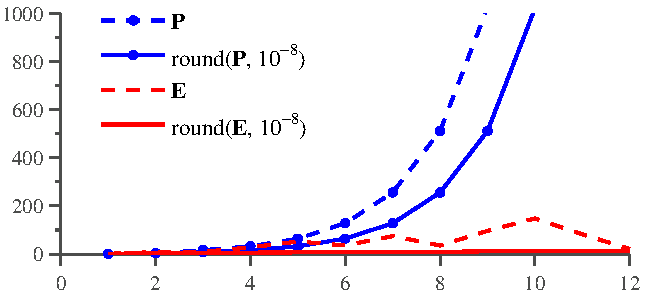
\includegraphics[width=12.0cm]{images/ranks_growth_temp=10,N=12,J=1_v2.pdf}
 \\
 & \parbox{12.3cm}{\centering\scriptsize размер решетки Изинга } \\
 \end{tabular}
 % \centerline{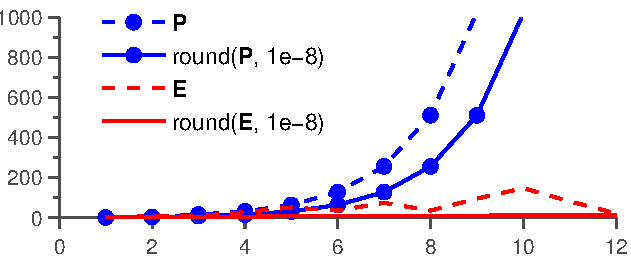
\includegraphics[width=\columnwidth]{figures/ranks_growth_temp=10,N=12,J=1}}
 \caption{Максимальный TT\hyp{}ранг тензора энергии~$\tens{E}$ и тензора ненормированной вероятности~$\widehat{\tens{P}}$ для гомогенной решетки Изинга с температурой равной~10 и весами парных потенциалов равными~$1$. Детали см. в разделе \ref{sec::exp1}. \label{fig:ranks-growth}}
 \end{center}
 \end{figure}


\subsection{Вычисление нормировочной константы~$Z$}
\label{sec:partition-function}
Естественный подход к подсчету нормировочной константы состоит в представлении всего тензора ненормированной вероятности~$\widehat{\tens{P}}$ в TT\hyp{}формате и в последующем суммировании всех его элементов. На практике тензор~$\widehat{\tens{P}}$ обладает экспоненциально большими TT\hyp{}рангами, и работа с его TT\hyp{}представлением становиться неэффективной. С другой стороны, каждый отдельный фактор графической модели можно точно представить в TT\hyp{}формате. В этом разделе предложен алгоритм подсчета нормировочный константы, который работает с TT\hyp{}представлением отдельных факторов~$\tensGreek{\Psi}_{\ell}$, не строя TT\hyp{}представление всего тензора~$\widehat{\tens{P}}$.

\subsubsection{Алгоритм}
Пусть все факторы графической модели уже представлены в TT\hyp{}формате~(см. раздел~\ref{sec:prob-representation}):
\begin{equation}
\tensGreek{\Psi}_{\ell}(\vec{x}^{\ell}) = \tensGreek{\Psi}_{\ell}(\vec{x}) = G^{\tensGreek{\Psi}_{\ell}}_1[x_1] \dotsm G^{\tensGreek{\Psi}_{\ell}}_n[x_n].
\end{equation}
Далее символ $G^{\ell}_k[x_k](\alpha^{\ell}_{k - 1}, \alpha^{\ell}_k)$ будет использоваться как сокращенное обозначение для $G^{\tensGreek{\Psi}_{\ell}}_k[x_k](\alpha^{\tensGreek{\Psi}_{\ell}}_{k - 1}, \alpha^{\tensGreek{\Psi}_{\ell}}_k)$.

По определению, нормировочная константа~$Z$ вычисляется как сумма значений ненормированного распределения на всех конфигурациях:
\begin{equation*}
Z = \sum_{\vec{x}} \prod_{\ell = 1}^{m} \underbrace{\tensGreek{\Psi}_{\ell}(\vec{x})}_{\text{$\in \mathbb{R}$}}
= \!\!\sum_{x_1, \dots, x_d} \bigotimes_{\ell = 1}^{m} \left (G^{\ell}_1[x_1] \dotsm G^{\ell}_d[x_d]  \right).
\end{equation*}
Второе равенство выполнено, т.~к. кронекерово произведение чисел (матриц размера $1 \times 1$) эквивалентно обычному произведению.


Пользуясь свойством смешанного произведения $AC \otimes BD = (A\otimes B)(C \otimes D)$, преобразуем выражение для~$Z$:
\begin{equation*}
Z =
\sum_{x_1, \dots, x_d} \left ( G^1_1[x_1] \otimes \dotsb \otimes G^m_1[x_1] \right ) \dotsm
\left ( G^1_d[x_d] \otimes \dotsb \otimes G^m_d[x_d] \right ).
\end{equation*}

Обозначим кронекерово произведение матриц~$G^\ell_k[x_k]$ через~$A_k[x_k]$:
\begin{equation*}
A_k[x_k] = G^1_k[x_k] \otimes \dotsb \otimes G^m_k[x_k].
\end{equation*}

Для любого значения~$x_k$ матрица~$A_k[x_k]$ имеет размеры $(\rank_{k - 1}(\tensGreek{\Psi}_1)  \dotsm  \rank_{k - 1}(\tensGreek{\Psi}_m)) \times (\rank_{k}(\tensGreek{\Psi}_1)  \dotsm  \rank_{k}(\tensGreek{\Psi}_m))$. Значение её элементов выражается через элементы матриц~$G_k^{\ell}[x_k]$:
\begin{multline*}
A_k[x_k](\alpha^1_{k - 1}, \dots, \alpha^m_{k - 1}; \alpha^1_i, \dots, \alpha^m_k) = G^1_k[x_k](\alpha^1_{k - 1}, \alpha^1_k)  \dotsm  G^m_k[x_k](\alpha^m_{k - 1}, \alpha^m_k).
\end{multline*}

Таким образом, матрица~$A_k[x_k]$ представлена в TT\hyp{}формате, а её TT\hyp{}ранг равен одному (т.~к. $G^{\ell}_k[x_k](\alpha^{\ell}_{k - 1}, \alpha^{\ell}_k)$ --- это матрица размера $1 \times 1$).

Представим нормировочную константу~$Z$ в виде произведения $d$~матриц:
\begin{multline*}
Z = \sum_{x_1, \dots, x_d}  A_1[x_1] \ldots  A_d[x_d]
= \left ( \sum_{x_1} A_1[x_1] \right ) \ldots  \left ( \sum_{x_d} A_d[x_d] \right ) = B_1 \dotsm  B_d,
\end{multline*}
где
\begin{equation*}
B_k = \sum_{x_k = 1}^{n_k} A_k[x_k].
\end{equation*}

TT\hyp{}преставление матрицы~$B_k$ можно получить просуммировав $n_k$ матриц в TT\hyp{}формате. Все матрицы~$B_k$ можно построить и держать в оперативной памяти, т.~к. TT\hyp{}ранги~$B_k$ не превосходят~$n_k$.

\begin{algorithm}[tb]
   \caption{Подсчет нормировочной константы~$Z$}
   \label{alg:Z-computing}
\begin{algorithmic}[1]
   \REQUIRE факторы $\tensGreek{\Psi}_1, \dots, \tensGreek{\Psi}_m$, точность округления $\varepsilon$
   \ENSURE оценка нормировочной константы $\widehat{Z}$
   \FOR{$\ell := 1$ \TO $m$}
   \STATE Найти TT\hyp{}ядра $G^{\ell}_1, \dots, G^{\ell}_d$ для тензора $\tensGreek{\Psi}_{\ell}$
   \ENDFOR
   \STATE Инициализировать $\vec{f}_{d + 1} := 1$
   \FOR{$k := d$ \TO $1$}
     \STATE Инициализировать $B_k := 0$
     \FOR{$x_k := 1$ \TO $n_k$}
       \STATE Построить TT\hyp{}матрицу $A_k[x_k] = \bigotimes_{\ell = 1}^m G^\ell_k[x_k]$
       \STATE $B_k := B_k + A_k[x_k]$
     \ENDFOR
     \STATE $\overline{\vec{f}_k} := B_k \cdot \vec{f}_{k + 1}$
     \STATE $\vec{f}_k := \round(\overline{\vec{f}_k}, \varepsilon)$
   \ENDFOR
   \STATE $\widehat{Z} := \vec{f}_1$
\end{algorithmic}
\end{algorithm}

Матрицы $B_1$ и $B_d$ являются вектором-строкой и вектором-столбцом соответственно, а значит результат произведения $B_1 \ldots B_d$~--- это число.
Построив TT\hyp{}матрицы~$B_k$, их можно перемножать, округляя результат после каждого умножения~(см. алгоритм~\ref{alg:Z-computing}). Параметр~$\varepsilon$ контролирует баланс между точностью и скоростью работы алгоритма.

Помимо нормировочной константы~$Z$, предложенный метод также позволяет найти маргинальные распределения на переменные графической модели. Ненормированное маргинальное распределение~$\hat{p}_k(x_k)$ вычисляется следующим образом:
$
\hat{p}_k(x_k) = B_1\ldots B_{k-1} A_k[x_k] B_{k+1}\ldots B_{d}.
$
При этом произведения~$B_1\ldots B_{k-1}$ и $B_{k+1}\ldots B_{d}$, $i=1,\ldots,n$ можно предрассчитать за $2 (d - 1)$ умножений TT\hyp{}матриц. Дополнительно рассчитав все произведения вида $B_i\ldots B_j$, $1 \leq i < j \leq n$, можно вычислять маргинальное распределение на любое подмножество переменных.

\subsubsection{Теоретический анализ алгоритма~\ref{alg:Z-computing}}
В этом разделе предоставлены теоретические гарантии точности оценки нормировочной константы алгоритмом~\ref{alg:Z-computing}.

Обозначим оценку произведения TT\hyp{}матриц~$\{B_j\}_{j = k}^d$ за~$\vec{f}_k$, $\vec{f}_k = B_d$, $\widehat{Z} = \vec{f}_1$. Умножая TT\hyp{}матрицу на TT\hyp{}вектор и применяя TT\hyp{}округление, получаем~$\vec{f}_k$
$$
\vec{f}_k = \round(B_k \vec{f}_{k + 1}, \varepsilon),
$$
где точность TT\hyp{}округления контролирует относительную точность по евклидовой норме\footnote{Алгоритм TT\hyp{}округления контролирует относительную точность тензоров по норме Фробениуса, но для векторов норма Фробениуса совпадает с $L_2$-нормой.}:
\begin{equation}
\label{main-algorithm-rounding-inequality}
\left \| B_k \vec{f}_{k + 1} - \vec{f}_k \right \|_2 \leq \varepsilon \left \| B_k \vec{f}_{k + 1} \right \|_2.
\end{equation}

Основной результат представлен в теореме~\ref{thm:mrf-main}, затем приведено следствие, которое легче интерпретировать.
\begin{theorem}
\label{thm:mrf-main}
	Для любого набора факторов~$\tensGreek{\Psi}_1, \ldots, \tensGreek{\Psi}_m$ и любого значения параметра точности округления~$\varepsilon \geq 0$ абсолютная ошибка оценки нормировочной константы, посчитанной алгоритмом~\ref{alg:Z-computing}, не превосходит:
	\begin{equation}
	\begin{aligned}
	\label{tough-abs-err-bound}
	&\left |Z - \widehat{Z}  \right | \leq
	\left \| B_1 \right \|_2 \dotsm \left \| B_{n-2} \right \|_2 \cdot \left \| B_{d-1} \vec{f}_d - \vec{f}_{d-1} \right \|_2 + \\
	&+\left \| B_1 \right \|_2 \dotsm \left \| B_{d-3} \right \|_2 \cdot \left \| B_{d-2} \vec{f}_{d-1} - \vec{f}_{d-2} \right \|_2 + \dotsb + \\
	&+\left \| B_1 \vec{f}_2 - \vec{f}_1 \right \|_2
	\end{aligned}
	\end{equation}
\end{theorem}

\begin{corollary}
\label{thm:mrf-corollary}
	Для любого набора факторов~$\tensGreek{\Psi}_1, \ldots, \tensGreek{\Psi}_m$ и любого значения параметра точности округления~$\varepsilon \geq 0$ абсолютная ошибка оценки нормировочной константы, посчитанной алгоритмом~\ref{alg:Z-computing}, не превосходит:
	\begin{equation}
		\label{epsilon-inequality}
		\left |Z - \widehat{Z}\right |  \leq \left \| B_1 \right \|_2 \dotsm \left \| B_d \right \|_2 ((1 + \varepsilon)^{d-1} - 1)
	\end{equation}
\end{corollary}
Оценка из следствия менее точная, но позволяет по требуемой итоговой точности выбрать достаточный~$\varepsilon$.

Чтобы воспользоваться результатами теоремы~\ref{thm:mrf-main}, необходимо вычислять 2-норму векторов и матриц в TT\hyp{}формате. 2-норма вектора совпадает с нормой Фробениуса соответствующего тензора, поэтому значения~$\left \| B_k \vec{f}_{k + 1} - \vec{f}_k \right \|_2$ легко вычисляются. Хотя подсчет 2-нормы матриц в TT\hyp{}формате является вычислительно сложной задачей, 2-норму можно оценить сверху с помощью нормы Фробениуса или с помощью эмпирически более точной оценки, использующей структуру матрицы~$B_k$:
\begin{equation}
\label{eq:l2computing}
\begin{aligned}
\left \| B_k \right \|_2 &= \left \| \sum_{x_i} G_k^1 [x_k] \otimes \dotsb \otimes G_i^m [x_k] \right \|_2 \leq
 \sum_{x_i} \left \| G_i^1 [x_k] \otimes \dotsb \otimes G_i^m [x_k] \right \|_2 =\\
& = \sum_{x_k} \left \| G_k^1 [x_k] \right \|_2 \dotsm \left \| G_i^m [x_k] \right \|_2=U_k.
\end{aligned}
\end{equation}
Здесь используется равенство: $\left \| A \otimes B \right \|_2 = \left \| A \right \|_2 \left \| B \right \|_2$.

 \begin{figure}
 \begin{center}
 \begin{tabular}{m{0.3cm}@{}m{12cm}}
 \begin{sideways}\parbox{4cm}{\centering\scriptsize   }\end{sideways}
 & 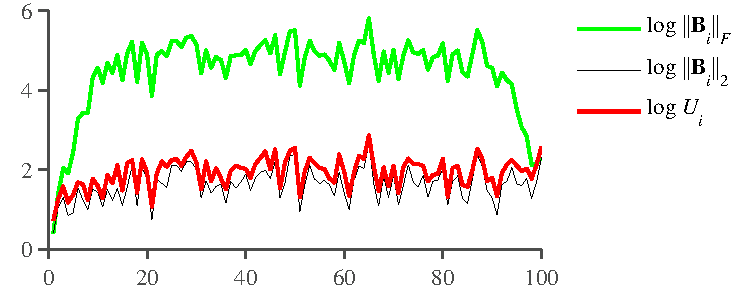
\includegraphics[width=12cm]{images/2norm.pdf}
 \\
 & \parbox{10.3cm}{\centering\scriptsize номер переменной~$k=1,\ldots,d$ } \\
 \end{tabular}
 \end{center}
 \caption{ Сравнение Фробениусовой и спектральной нормы матрицы~$B_k$ с верхней оценкой~$U_k$. График построен для модели Изинга с решеткой размера $10 \times 10$, в которой коэффициенты унарных и парных потенциалов сгенерированы из равномерного распределения на $[-1, 1]$, а температура равна~$1$.
 \label{fig:zUpperBound}}
 \end{figure}
 На рис.~\ref{fig:zUpperBound} представлены результаты сравнения величины нормы Фробениуса~$\|B_k\|_F$, спектральной нормы~$\|B_i\|_2$ и её верхней оценки~$U_k$. Значения разных норм указаны для всех индексов~$i = 1, \ldots, n$ фиксированной модели Изинга.



 \begin{figure}
 \begin{center}
 \begin{tabular}{m{0.3cm}@{}m{12cm}}
 \begin{sideways}\parbox{4cm}{\centering\scriptsize  $\log Z$ }\end{sideways}
 & 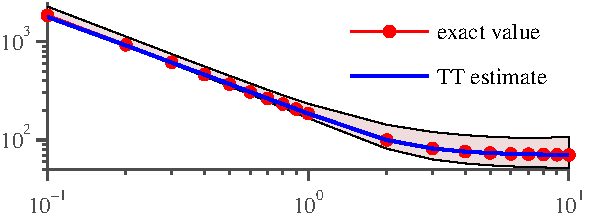
\includegraphics[width=12cm]{images/10x10,J=1,average=10,confInt_v3.pdf}
 \\
 & \parbox{12.3cm}{\centering\scriptsize температура~$T$} \\
 \end{tabular}
 \end{center}
 \caption{Доверительный интервал на значение нормировочной константы~$Z$, полученный из теоремы~\ref{thm:mrf-main} и неравенства~\eqref{eq:l2computing}. Детали см. в разделе \ref{sec::expZ}.  \label{fig:zConf}}
 \end{figure}


\subsubsection{Доказательство теоремы~\ref{thm:mrf-main}}

\begin{lemma}
\label{app:proof-of-theorem-2:lemma}
В условиях теоремы~\ref{thm:mrf-main} для всех индексов $k = 1, \ldots, d - 1$ верно следующее неравенство:
\begin{equation}
\begin{aligned}
\label{app:proof-of-theorem-2:lemma:inequality}
&\left\| B_k \ldots B_d - \vec{f}_k \right\|_2 \leq
\left\| B_k \right\|_2 \ldots \left\| B_{d - 2} \right\|_2 \cdot \left\| B_{d - 1}\vec{f}_d - \vec{f}_{d - 1}\right\|_2 + \\
 &+ {} \left\| B_k \right\|_2 \ldots \left\| B_{d - 3} \right\|_2 \cdot \left\| B_{d - 2}\vec{f}_{d - 1} - \vec{f}_{d - 2} \right\|_2 +
{} \ldots + \left\| B_k\vec{f}_{k + 1} - \vec{f}_k \right\|_2.
\end{aligned}
\end{equation}
\end{lemma}

\begin{proof}
Проведем доказательство по индукции.

В качестве базы индукции рассмотрим $k = d - 1$:
\begin{equation*}
\left\| B_{d - 1}B_d - \vec{f}_{d - 1} \right\|_2 = \left\| B_{d - 1}\vec{f}_d - \vec{f}_{d - 1} \right\|_2.
\end{equation*}
(т.~к. $\vec{f}_d = B_d$ по построению.)

Предположим теперь, что~(\ref{app:proof-of-theorem-2:lemma:inequality}) верно $\forall k = j + 1, \ldots, d - 1$. Тогда для $k = j$ получаем
\begin{align*}
&\left\| B_j \ldots B_d - \vec{f}_j \right\|_2 = \\
& = \left\| (B_j \ldots B_d - B_j\vec{f}_{j + 1}) + (B_j\vec{f}_{j + 1} - \vec{f}_j) \right\|_2 \leq \\
& \leq \left\| B_j \right\|_2 \left\| B_{j + 1} \ldots B_d - \vec{f}_{j + 1} \right\|_2 + \left\| B_j\vec{f}_{j + 1} - \vec{f}_j \right\|_2 \leq \\
&\leq \left\| B_j \right\|_2 (
\left\| B_{j + 1} \right\|_2 \ldots \left\| B_{d - 2} \right\|_2 \cdot \left\| B_{d - 1}\vec{f}_d - \vec{f}_{d - 1}\right\|_2 + \\
& + \left\| B_{j + 1} \right\|_2 \ldots \left\| B_{d - 3} \right\|_2 \cdot \left\| B_{d - 2}\vec{f}_{d - 1} - \vec{f}_{d - 2} \right\|_2 +  \\
& + \ldots + \left\| B_{j + 1}\vec{f}_{j + 2} - \vec{f}_{j + 1} \right\|_2
) + \left\| B_j\vec{f}_{j + 1} - \vec{f}_j \right\|_2.
\end{align*}
Таким образом, (\ref{app:proof-of-theorem-2:lemma:inequality}) верно для~$k = j$.
\end{proof}

\begin{proof}[Доказательство теоремы~\ref{thm:mrf-main}]
По построению, $Z = B_1 \ldots B_d$, а $\widehat{Z} = \vec{f}_1$. Таким образом, выполнены равенства
\begin{equation*}
\label{app:proof-of-theorem-2:difference-as-matrix-norm}
|Z - \widehat{Z}| = |B_1 \ldots B_d - \vec{f}_1| = \left\| B_1 \ldots B_d - \vec{f}_1 \right\|_2.
\end{equation*}
Здесь используется тот факт, что $B_1 \ldots B_d$ и $\vec{f}_1$ --- числа, а для чисел модуль совпадает с $L_2$-нормой одноэлементного вектора. Для завершения доказательства осталось применить лемму~\ref{app:proof-of-theorem-2:lemma} к полученному выражению.
\end{proof}

\subsection{Доказательство следствия~\ref{thm:mrf-corollary}}

\begin{lemma}
\label{app:proof-of-corollary-of-theorem-2:lemma-for-f}
В условиях следствия~\ref{thm:mrf-corollary} для всех индексов $i = 1, \ldots, d$ верно следующее неравенство:
\begin{equation}
\label{app:proof-of-corollary-of-theorem-2:lemma-for-f:inequality}
\left\| \vec{f}_k \right\|_2 \leq \left\| B_k \right\|_2 \ldots \left\| B_d \right\|_2 (1 + \varepsilon)^{d - k}.
\end{equation}
\end{lemma}
\begin{proof}
Проведем доказательство по индукции.

Для $k = n$ утверждение следует из определения~$\vec{f}_d$.

Пусть~(\ref{app:proof-of-corollary-of-theorem-2:lemma-for-f:inequality}) верно $\forall j = k + 1, \ldots, d$. Тогда из~(\ref{main-algorithm-rounding-inequality}) следует, что
\begin{align*}
\left\| \vec{f}_j \right\|_2 = &\left\| \vec{f}_j - B_j\vec{f}_{j + 1} + B_j\vec{f}_{j + 1} \right\|_2 \leq \\
\leq & ~ \varepsilon \left\| B_j \right\|_2 \left\| \vec{f}_{j + 1} \right \|_2 + \left\| B_j \right\|_2 \left\| \vec{f}_{j + 1} \right \|_2 = \\
 = &\left\| B_j \right\|_2 \left\| \vec{f}_{j + 1} \right \|_2 (1 + \varepsilon).
\end{align*}
Чтобы завершить доказательство, остаётся воспользоваться предположением индукции для~$\left\| \vec{f}_{j + 1} \right \|_2$.
\end{proof}

\begin{lemma}
\label{app:proof-of-corollary-of-theorem-2:lemma-for-difference}
В условиях следствия~\ref{thm:mrf-corollary} для всех индексов $k = 1, \ldots, d - 1$ верно следующее неравенство:
\begin{equation}
\label{app:proof-of-corollary-of-theorem-2:lemma-for-difference:inequality}
\left\| B_k \vec{f}_{k + 1} - \vec{f}_k \right\|_2 \leq \left\| B_k \right\|_2 \ldots \left\| B_d \right\|_2 \varepsilon (1 + \varepsilon)^{d - k - 1}.
\end{equation}
\end{lemma}
\begin{proof}
Утверждение следует из леммы~\ref{app:proof-of-corollary-of-theorem-2:lemma-for-f} и неравенства
\begin{equation*}
\left\| B_k \vec{f}_{k + 1} - \vec{f}_k \right\|_2 \leq \varepsilon \left\| B_k \vec{f}_{k + 1} \right\|_2 \leq \varepsilon \left\| B_k \right\|_2 \left\| \vec{f}_{k + 1} \right\|_2,
\end{equation*}
которое в свою очередь следует из~(\ref{main-algorithm-rounding-inequality}).
\end{proof}


\begin{proof}[Доказательство следствия~\ref{thm:mrf-corollary}]
Применяя лемму~\ref{app:proof-of-corollary-of-theorem-2:lemma-for-difference} к неравенству~(\ref{tough-abs-err-bound}), получаем
\begin{align*}
&|Z - \widehat{Z}| \leq \left\| B_1 \right\|_2 \ldots \left\| B_d \right\|_2 \varepsilon +
\left\| B_1 \right\|_2 \ldots \left\| B_d \right\|_2 \varepsilon (1 + \varepsilon) + \ldots + \\
&+ \left\| B_1 \right\|_2 \ldots \left\| B_d \right\|_2 \varepsilon (1 + \varepsilon)^{d - 2} =
\left\| B_1 \right\|_2 \ldots \left\| B_d \right\|_2 \varepsilon (1 + (1 + \varepsilon) + \ldots + (1 + \varepsilon)^{d - 2}).
\end{align*}
Пользуясь формулой суммы геометрической прогрессии $1 + (1 + \varepsilon) + \ldots + (1 + \varepsilon)^{d - 2} = ((1 + \varepsilon)^{d - 1} - 1) / \varepsilon$, получаем~(\ref{epsilon-inequality}).
\end{proof}

%\section{Поиск минимума энергии}
%Описание актуальности задачи -- что нужно искать минимумы, причем желательно несколько разных.
%\subsection{Метод решения блочных задач на собственные значения}
%\alert{рассказать про riemannian LOBPCG}
